\documentclass[10pt]{beamer}
\usepackage{etex}
\usepackage[utf8x]{inputenc}
\usepackage[ngerman]{babel}
\usepackage{bbm}

\usepackage{tabularx}
\usepackage{graphicx}
\usepackage{url}
\usepackage{listings}

\setbeamertemplate{bibliography item}{[\theenumiv]}

\newif\ifzihbackground
\zihbackgroundtrue
%\zihbackgroundfalse
             %\hspace*{3.0mm}\color{darkblue}
\includegraphics[height=7.81mm]{logo/tu_logo_black}\hspace{67.0mm}\hline
% Yes, this is dirty
\newcommand\zihmaketitle{
	\definecolor{white}{gray}{1.00}%
	\setbeamercolor{normaltext}{bg=darkblue}%
	\setbeamertemplate{headline}{%
		\vskip6.15mm\color{white}\setlength{\arrayrulewidth}{0.3pt}%
		\begin{tabular*}{\paperwidth}[b]{l@{\extracolsep\fill}}%
			\hspace*{3.0mm}\color{white}%
            
\includegraphics[height=7.81mm]{theme/logo/tu_logo_black}\hspace{67.0mm}\\[1.2mm]
			\hline\hspace*{11.76mm}\rule[-0.8mm]{0pt}{2.47mm}%
			\def\@@dummyComma{}\rule{0pt}{5.8pt}%
			\insertinstitute \\%
			\hline%
		\end{tabular*}%
		\hspace{-\paperwidth}%
	}%
    \ifzihbackground
      \setbeamertemplate{footline}{}
      \setbeamertemplate{background}{
\includegraphics[height=\paperheight,width=\paperwidth]{theme/logo/bg}}
      \else
      \setbeamertemplate{footline}{
          \parbox[t][22mm]{\paperwidth}{
              \vspace*{-8.18mm}
              \rule
              {98.6mm}{0pt}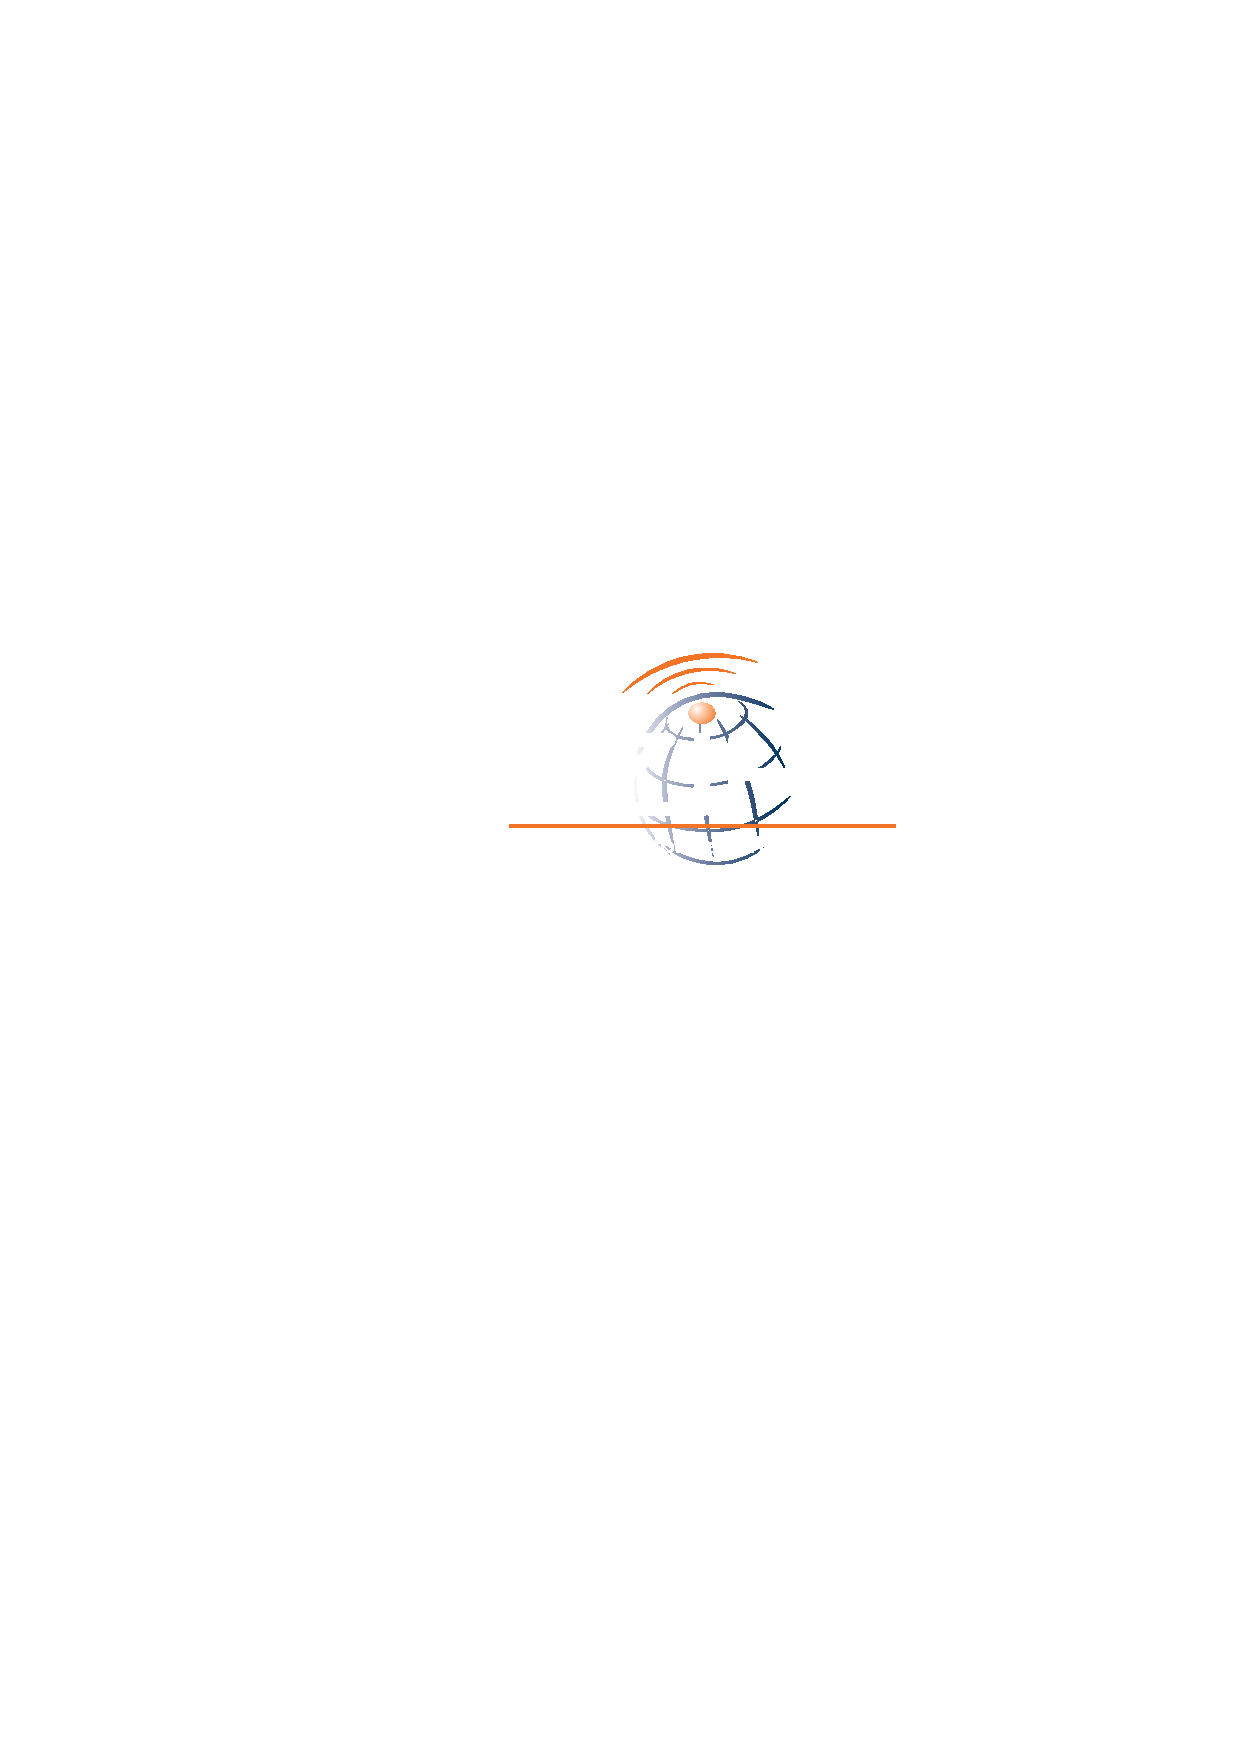
\includegraphics[height=15mm]{theme/logo/zih_logo_white}

          }
      }
    \fi%
   \frame{\titlepage}
    % Kopf-/Fusszeilen fuer restliche Folien
    \setbeamercolor{normal text}{bg=white}
    \setbeamertemplate{background}{}
    \setbeamertemplate{headline}[zih01 theme]
    \setbeamertemplate{footline}[zih01 theme]
}

\usetheme{Dresden}
%\useoutertheme{theme/zih01}
%\useinnertheme{theme/zih01}
\usepackage{theme/beamerouterthemezih01}
\usepackage{theme/beamerinnerthemezih01}

%\useinnertheme{rounded}
\definecolor{darkblue}{rgb}{0.04, 0.16, 0.32}
% font color for headlines etc.
\setbeamercolor*{structure}{fg=darkblue,bg=white}
% disable navigation symbols
\setbeamertemplate{navigation symbols}{}
% can't remember what this is good for
\setbeamercovered{transparent}

% reduce margin size
\setbeamersize{text margin left=0.7cm}
\setbeamersize{text margin right=0.7cm}
%
% Outer Color Theme "whale" sorgt f?r strenge farbliche Trennen zwischen Zierrat
% und dem eigentlichen Inhalt. Ein dunkler Hintergrund f?r den Folientitel wirkt
% aber zu aufdringlich.
%
\usecolortheme{orchid}
%\setbeamercolor{titlelike}{parent=structure}

%
% Inner Color Theme "orchid" sorgt f?r farblich abgesetzt Bl?cke (Definitionen,
% S?tze, Beispiele, Beweise, ...).
%
%\usecolortheme{orchid}

%zum drucken
%\usepackage{pgfpages}
%\pgfpagesuselayout{resize to}[a4paper,border shrink=5mm,port]
%\pgfpagesuselayout{4 on 1}[a4paper,border shrink=3mm, landscape]

%%%%%%%%%%%%%%%%%%%%%%%%%%%%

\definecolor{LightGray}		{gray}{0.9}
\definecolor{Gray}		{gray}{0.5}
\definecolor{DarkGray}     	{gray}{0.2}
\definecolor{listinggray} 	{gray}{0.96}
\definecolor{DarkGreen}     	{rgb}{0.0,0.6,0.0}
\definecolor{DarkRed}     	{rgb}{0.6,0.0,0.0}
\definecolor{DarkBlue}     	{rgb}{0.0,0.0,0.6}
\definecolor{DarkCyan}     	{rgb}{0.7,0.7,0.2}
\definecolor{DarkDarkGreen}	{rgb}{0.0,0.4,0.0}

\lstset{language=C}
\lstset{linewidth=0.99\textwidth}
%\lstset{boxpos=c}
\lstset{xleftmargin=0.03\textwidth}
%\lstset{breaklines=true}
\lstset{framexleftmargin=0.03\textwidth}
\lstset{abovecaptionskip=\smallskipamount}
\lstset{belowcaptionskip=\smallskipamount}
\lstset{basicstyle=\ttfamily\tiny}
\lstset{backgroundcolor=\color{listinggray}}
%\lstset{frameround=ffff}
%\lstset{frame=shadowbox}
%\lstset{rulesepcolor=\color{Gray}}
\lstset{numbers=left}
\lstset{numberstyle=\tiny \color{DarkGray}}
\lstset{numbersep=0.01\textwidth}
\lstset{showstringspaces=false}
%\lstset{showspaces=false}
\lstset{tabsize=4}

%% all words in the following list are printed in bold letters in a listing 
\lstset{emph={__asm__, __volatile__, return, main,},emphstyle={\bfseries\color{DarkGray}}}
\lstset{captionpos=b}

% Style für C Sourcecode
\lstdefinestyle{CA}{
        language=C,
        basicstyle=\ttfamily\scriptsize,
        keywordstyle=\ttfamily\bfseries\color{DarkBlue},
        stringstyle=\ttfamily\color{DarkRed},
        commentstyle=\ttfamily\color{DarkGreen},
        identifierstyle=\ttfamily\color{DarkCyan},
        backgroundcolor=\color{listinggray},
}

%%%%%%%%%%%%%%%%%%%%%%%%%%%%


\newcommand{\mq}[1]{\glqq#1\grqq}

\newcommand{\backupbegin}{
    \newcounter{finalframe}
    \setcounter{finalframe}{\value{framenumber}}
}
\newcommand{\backupend}{
    \setcounter{framenumber}{\value{finalframe}}
}
% registered, copyright und trademark zeichen
\def\TReg{\textsuperscript{\textregistered}}
\def\TCop{\textsuperscript{\textcopyright}}
\def\TTra{\textsuperscript{\texttrademark}}

\newcommand\Small{\fontsize{9}{9.0}\selectfont}
\newcommand*\LSTfont{\Small\ttfamily}

\date{8. Februar 2016}
\institute[ZIH TUD]{Zentrum f\"{u}r Informationsdienste und Hochleistungsrechnen -- TU Dresden}
\title[LCTP]{Vorstellung Workpackage 3 ADA-FS}
\subtitle{ADA-FS Kick-Off}
\author[Oeste]{Sebastian Oeste}

\room{WIL A315}
\address{Zellscher Weg 12}
\city{Dresden}
\phone{+49 351 463-32041}
\email{sebastian.oeste@tu-dresden.de}
\xmpp{soeste@tu-dresden.de}

\setbeamercovered{transparent}

%\captionsetup[figure]{labelformat=empty} needs \usepackage{caption}

\begin{document}
\zihmaketitle
\begin{frame}{Gliederung}
    \tableofcontents
\end{frame}

\section{Arbeitspaket 3.1}

\begin{frame}{Topology Discovery and Dynamic Resource Tracking}
    \begin{itemize}
        \item Erfassen der Ressourcen, die auf dem HPC-System zur Verf\"{u}gung
            stehen.
        \item Bereitstellen einer \emph{System-Map} aller Compute-Nodes und
            Speicherkomponenten \emph{(statische Komponente)}.
        \item Darstellung dynamisch genutzter (geteilter) Ressourcen von parallelen
            Anwendungen \emph{(dynamische Komponente)}.
    \end{itemize}
    \begin{block}{Ziel:}
        Die Differenz aus der \emph{System-Map} und der dynamischer Ressourcen-Auslastung
        sind die Ressourcen, die tats\"{a}chlich zur Verf\"{u}gung stehen.
    \end{block}
\end{frame}

\subsection{Topology Discovery}

\begin{frame}{System-Map}
    \begin{block}{System-Map}
        Die System-Map soll einen \"{U}berblick \"{u}ber die HPC-Plattform
        und die zur Verf\"{u}gung stehenden Ressourcen der Plattform bieten.
    \end{block}
    \begin{itemize}
        \item Compute-Nodes mit Anzahl der Cores.
        \item Verf\"{u}gbarer Arbeitsspeicher pro Knoten.
        \item Verf\"{u}gbarer lokaler Speicher (HDD, SSD, NVRAM).
        \item Zentrales Dateisystem mit verf\"{u}gbaren Netzbandbreiten.
        \item Bandbreite zwischen den Compute-Nodes.
    \end{itemize}
\end{frame}

\begin{frame}{Umsetzung via SLURM}
    Umfangreiche Plugin-Architektur z.\,B.\,:
    \begin{itemize}
        \item Topology-Plugins % TODO: links!
        \item Node-Selection-Plugins
    \end{itemize}
    Slurm speichert die Topologie in einer Datei /etc/slurm/topology.conf.\\
    Bietet Informationen zu:
    \begin{itemize}
        \item Anzahl Compute-Nodes
        \item Anzahl Switches
        \item Verbindung zwischen Switches und Compute-Nodes
    \end{itemize}
    \begin{block}{\href{http://slurm.schedmd.com/topology.html}{Topology Guide}}
        At some point in the future Slurm code may be provided to gather network
        topology information directly. Now the network topology information must be
        included in a topology.conf configuration file\ldots
    \end{block}
    \tiny{\footnote{http://slurm.schedmd.com}}
\end{frame}


\begin{frame}{hwloc - The portable Hardware Locality}

    Open-MPI Projekt: Bibliothek und Tools.\\
    Umfasst CLI und C-API.

    \begin{itemize}
    \item Sammelt alle verf\"{u}gbaren Informationen vom OS.
    \item Erstellt abstrakten Baum von Objekten z.B.\,: memory nodes, caches,
        processors, sockets, processor cores, \ldots
    \item Lokalit\"{a}t von I/O devices z.B.\,: network interfaces, Infiniband HCAs
        oder GPUs.
    \item PCI Ger\"{a}te Erkennung z.B.\,: OpenCL, CUDA und Xeon Phi
        Beschleuniger.
    \end{itemize}


    In vielen Projekten bereits genutzt.\\
    \begin{itemize}
        \item PaRSEC
        \item StarPU
        \item TORQUE - resource manager
        \item likwid
    \end{itemize}

    %The hwloc core gathers all the available pieces of information from the
    %operating system and builds an abstracted, portable tree of objects: memory
    %nodes (and node groups), caches, processor sockets, processor cores,
    %hardware threads, and so on.

    %The entire tree of objects is presented in a cross-linked data structure; the
    %tree can be traversed via children, parents, siblings, and cousins.

    %It also gathers various system attributes such as cache and memory
    %information as well as the locality of I/O devices such as network
    %interfaces, InfiniBand HCAs or GPUs.

    %Additionally hwloc can detect the locality PCI devices as well as OpenCL,
    %CUDA and Xeon Phi accelerators, network and InfiniBand interfaces, etc.

\end{frame}


\begin{frame}{hwloc - The portable Hardware Locality}

    \begin{figure}
        \centering
        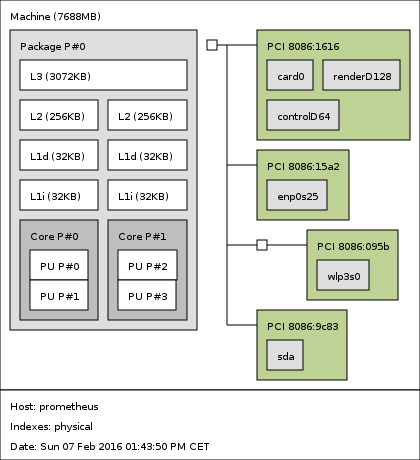
\includegraphics[width=0.58\textwidth]{fig/prometheus.png}
    \end{figure}
\end{frame}


\begin{frame}{netloc - Network Locality}

    Open-MPI Projekt.\\
    Erm\"{o}glicht Informationen \"{u}ber die Netzwerktopologie von HPC-Clustern zu identifizieren.
    \begin{itemize}
        \item Abstrakte Representation als Graph.
        \item Unterst\"{u}tzung f\"{u}r Ethernet und Infiniband Netzwerke.
        \item In Kombination mit \emph{hwloc} umfassende Sicht der Komponenten
            verschiedener Knoten und dem dazwischen liegendem Netzwerk.
    \end{itemize}

    %Additionally, by combining the hwloc single-server topology data with the
    %network topology data, netloc provides developers with a comprehensive view
    %of the HPC system topology, spanning from the processor cores in one server
    %all the way to the cores in another – including the complex network(s) in
    %between.

    %This first public release of the netloc project includes support for
    %OpenFlow-managed Ethernet and InfiniBand networks

\end{frame}


\begin{frame}{netloc - Network Locality}
    \begin{figure}
        \centering
        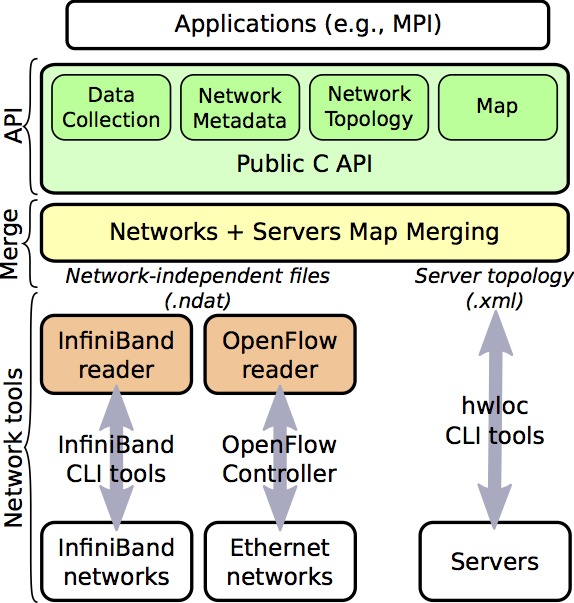
\includegraphics[width=0.58\textwidth]{fig/netloc-design.png}
    \end{figure}
    \tiny{\href{netloc}{https://www.open-mpi.org/projects/netloc/netloc-design-full-size.png}}
\end{frame}


%Starting with hwloc 2.0, both netloc and hwloc are distributed in hwloc releases.

\begin{frame}{Vorschlag}
    \begin{itemize}
        \item Entwicklung eines Tools auf Basis von hwloc und netloc zum
            identifizieren der Topologie.
        \item Einfaches Interface zum Abfragen der Informationen (einfach integrierbar).
        \item Unterst\"{u}tzung mehrerer Ausgabeformate z.B. als OTF2
            Stystem-Tree.
    \end{itemize}
    %(output als OTF2 System-Tree)
\end{frame}

\section{Arbeitspaket 3.2}

\subsection{Dynamic Resource Usage Tracking}

\begin{frame}{Dynamische Ressourcen Auslastung}
    \begin{block}{Dynamische Ressourcen Auslastung}
        Aktuelle Auslastung der Ressourcen einer Menge von Knoten.\\
        Wie hoch ist die Ressourcen Auslastung einer Anwendung?
    \end{block}
    \begin{itemize}
        \item Auslastung von Arbeitsspeicher und lokalen Speicher, pro Knoten
            oder NUMA-Domain.
        \item Lastmessung zwischen Zentralen Dateisystem und Compute-Node.
        \item Auf\"{u}hrung, nebenl\"{a}ufig zur Anwendung.
        \item Der Anwendungscode soll nicht ver\"{a}ndert werden.
    \end{itemize}
\end{frame}


\begin{frame}{perf}

    \begin{itemize}
        \item Events Subsystem im Linux-Kernel.
        \item Instrumentiert Hardware Performance Counter, tracepoints, KProbes,
            UProbes.
        \item geringer Overhead.
    \end{itemize}

\end{frame}

\begin{frame}{perf}

    \begin{figure}
        \centering
        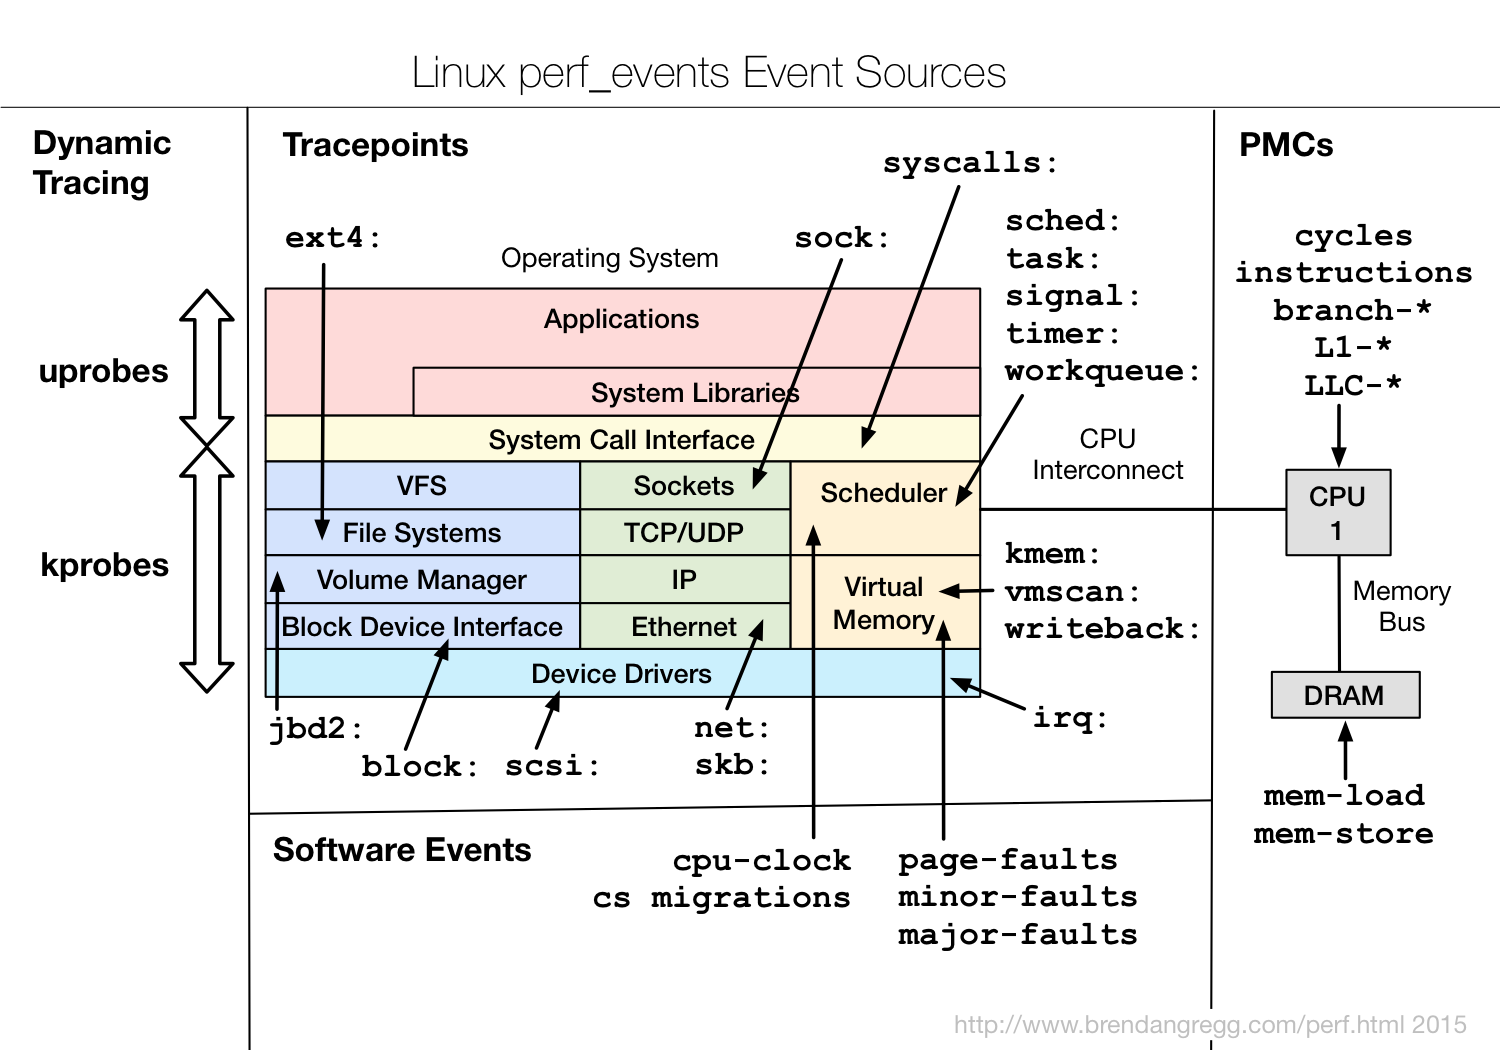
\includegraphics[width=0.79\textwidth]{fig/perf_events_map.png}
    \end{figure}
    \tiny{\href{perf}{http://www.brendangregg.com/perf\_events/perf\_events\_map.png}}
\end{frame}

\subsection{Integrated Monitoring}

\begin{frame}{Integrated Monitoring of the Ad-hoc File System}
    \begin{itemize}
        \item Integration der Monitoring Komponenten in das Ad-hoc Dateisystem.
        \item \"{U}berwachen von I/O Aufrufen an vier Schnittstellen.
            \begin{enumerate}
                \item Aufrufe von der Anwendung an das Dateisystem.
                \item Aufrufe des Ad-hoc Dateisystems zum unterliegenden Dateisystem.
                \item Anfragen vom \emph{data transfer executor}.
                \item Interner Datentransfer innerhalb des Ad-hoc Dateisystems.
            \end{enumerate}
        \item Aufgezeichnete I/O-Events werden in einer Datenbank gespeichert.
    \end{itemize}

    \begin{block}{Ziel}
        Analyse des Ad-hoc Dateisystems.
        Entwickelte Komponenten bieten Informationen zur Entwicklung und Optimierung des Systems.
    \end{block}
\end{frame}

\section{Arbeitspaket 3.3}

\subsection{Access Monitoring}

\begin{frame}{Access Monitoring through Applications}
    \begin{itemize}
        \item Monitoring von Datenzugriffen
        \item Wie oft kann eine I/O Anfrage lokal bearbeitet werden?
        \item Wie oft muss f\"{u}r eine I/O Anfrage kommuniziert werden?\\
            Wieviel zus\"{a}tzliche Zeit wird daf\"{u}r ben\"{o}tigt?
        \item Welche Dateien oder Dateisystembl\"{o}cke, werden
            von welchen Prozessen oder Knoten zugegriffen?
    \end{itemize}
    \begin{block}{Ziel}
        Diese Informationen stellen den Input f\"{u}r das "Data-Placement" da.
        Die Ergebnisse werden "pro Anwendungs-Lauf" gespeichert.
        Das Format soll einfach aggregierbar sein und in einer Datenbank gespeichert
        werden.
    \end{block}
\end{frame}


\begin{frame}{eBPF - extended Berkley Packet Filter}
    \begin{itemize}
        \item virtuelle Maschine innerhalb des Kernels
        \item BPF Programm wird aus dem User-Space geladen.
        \item Just-in-Time Compiler konvertiert BPF Code in nativen Bytecode.
        \item Ausf\"{u}hrung h\"{a}ngt an einem KProbe oder UProbe.
        \item abgefragte Daten werden in den User-Space kopiert
        \item ben\"{o}tigt aktuellen Kernel
    \end{itemize}
\end{frame}

\begin{frame}{eBPF - extended Berkley Packet Filter}
    \begin{figure}
        \centering
        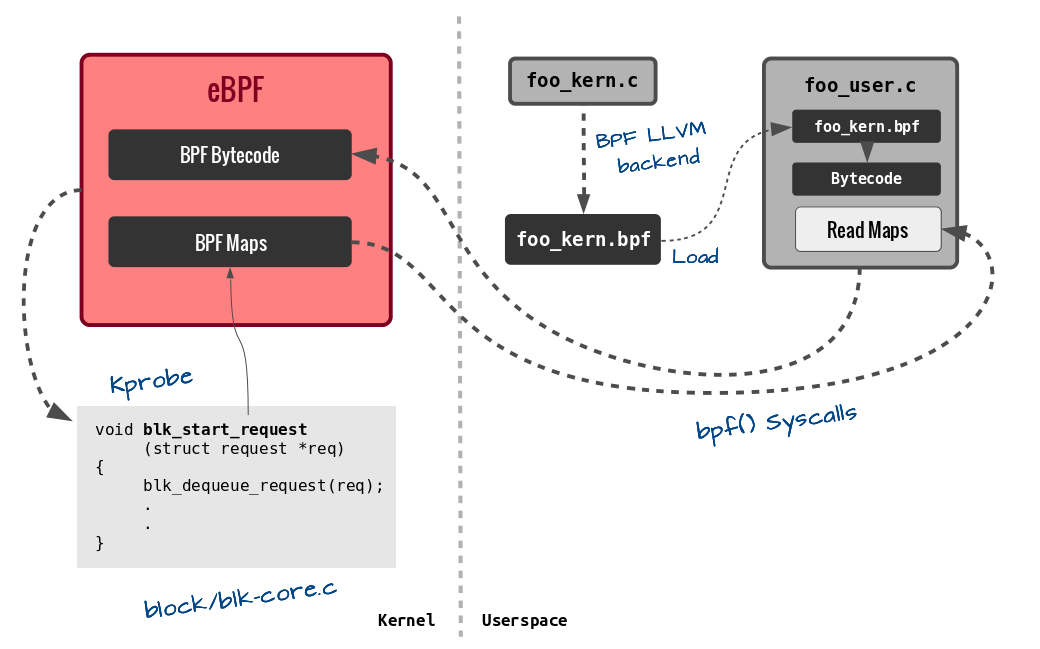
\includegraphics[width=0.98\textwidth]{fig/ebpf-session.png}
    \end{figure}
    \tiny{\href{eBPF}{https://suchakra.files.wordpress.com/2015/08/ebpf-session.png}}
\end{frame}

\begin{frame}{Workflow: Monitoring}
    \begin{enumerate}
        \item Eintrag pro Anwendungslauf.
        \item Abfragen der Informationen \"{u}ber Monitoring-Schnittstellen.
        \item Speichern in der Datenbank.
        \item Aggregationen in der Datenbank.
    \end{enumerate}
\end{frame}

\subsection{Monitoring Visualization}

\begin{frame}{Auswertung}
    \begin{itemize}
        \item Tools zur Datenbankabfrage der Monitoring Daten.
        \item Support f\"{u}r verschiedene Ausgabeformate.
        \item Visualisierung der Daten.
    \end{itemize}
\end{frame}


\end{document}
